\documentclass[french]{article}
\usepackage[T1]{fontenc}
\usepackage[utf8]{inputenc}
\usepackage{lmodern}
\usepackage[a4paper]{geometry}
\usepackage{babel}
\usepackage{amsmath}
\usepackage{amssymb}
\usepackage{graphicx}

\newcommand{\uconcat}{\ensuremath{+\!\!\!+\,}}

\DeclareMathOperator{\proj}{\pi}
\DeclareMathOperator{\sel}{\sigma}
\DeclareMathOperator{\frag}{frag}
\DeclareMathOperator{\defrag}{defrag}
\DeclareMathOperator{\crypt}{crypt}
\DeclareMathOperator{\decrypt}{decrypt}
\DeclareMathOperator{\group}{group}
\DeclareMathOperator{\id}{id}
\DeclareMathOperator{\dom}{dom}

\newcommand\typeT[1]{\text{\ttfamily #1}}
\newcommand{\decryptArgs}[2]{\decrypt_{\typeT{#1}, #2}}
\newcommand{\cryptArgs}[2]{\crypt_{#1 , \typeT{#2}}}
\newcommand{\projDelta}{\proj_{\delta}}
\newcommand{\selP}{\sel_p}
\newcommand{\decryptCAlpha}{\decryptArgs{c}{a}}
\newcommand{\cryptCAlpha}{\cryptArgs{\alpha}{c}}
\newcommand{\ch}{\typeT{c}}
\newcommand{\chp}{\typeT{c'}}
\newcommand{\groupDelta}{\group_{\delta}}
\newcommand{\fragDelta}{\frag_{\delta}}


\begin{document}
J'ai trouvé deux erreurs dans les lois algébriques
énoncées jusqu'à maintenant pour C2QL.

La première est probablement une erreur d'étourderie
au moment d'écrire la loi.

La deuxième, par contre, est une erreur dans la condition
d'application de la loi.


\section*{Loi (3), page 30 de la thèse}
\subsection*{Ce qui est écrit dans la thèse}
$$ 
\proj_{a_1} \circ \dots \circ \proj_{a_n} 
\equiv \proj_{a_1, \dots, a_n}
$$

\subsection*{Contre-exemple}
Si on considère la relation r suivante
\begin{center}
	\begin{tabular}{lr}
		a\(_{\text{1}}\) & a\(_{\text{2}}\)\\
		\hline
		a & 1\\
		b & 2\\
	\end{tabular}
\end{center}
son image par \(\pi_{a_2}\) est
\begin{center}
	\begin{tabular}{r}
		a\(_{\text{2}}\)\\
		\hline
		1\\
		2\\
	\end{tabular}
\end{center}
dont l'image par \(\pi_{a_1}\) est la table vide

Ainsi, l'image de r par
\(\pi_{a_1} \circ \pi_{a_2}\) est la table vide.

Par contre, l'image de r par
\(\pi_{a_1, a_2}\)
est la table r elle-même,
qui est différente de la table vide.



\subsection*{Correction}
La composition des projections correspond à la projection sur \emph{l'intersection},
et non pas à une projection sur l'union.

$$
\proj_{\delta_1} \circ \dots \circ \proj_{\delta_n} 
\equiv \proj_{\delta_1 \cap \dots \cap \delta_n}
$$

\section*{Lois (14) et (15) de l'article A Language for the Composition of Privacy-Enforcement Techniques}
\subsection*{Ce qui est écrit dans l'article}
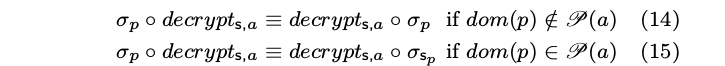
\includegraphics[width = .9\textwidth]{lois14-15.png}

\subsection*{Contre-exemple}
Le chiffrement pris pour l'exemple est artificiel, pour privilégier la simplicité de l'exemple. \\

On prend pour prédicat p 
$$p: a_1 + a_2 < 10$$ 

pour fonction de chiffrement s
$$ s: n \mapsto n + 50 $$

et pour ensemble des attributs chiffrés a
$$ a = \{a_1\} $$

Le domaine de $p$ est alors $\{a_1, a_2\}$
qui n'est pas une partie de $a$.
On est donc dans les hypothèses mentionnées
dans l'article pour la loi (14)

On s'intéresse à la relation r
\begin{center}
	\begin{tabular}{rr}
		a\(_{\text{1}}\) & a\(_{\text{2}}\)\\
		\hline
		51 & 2\\
	\end{tabular}
\end{center}

L'image de r par
$\sel_p \circ \decryptArgs{s}{a_1}$
est la relation
\begin{center}
	\begin{tabular}{rr}
		a\(_{\text{1}}\) & a\(_{\text{2}}\)\\
		\hline
		1 & 2\\
	\end{tabular}
\end{center}

L'image de r par
$\decryptArgs{s}{a_1} \circ \sel_p$
est la relation vide.

Ainsi donc, la relation (14)
dans l'article est fausse
car la condition donnée n'est pas assez restrictive.

\subsection*{Correction possible}
Ce problème est résolu si on s'intéresse à l'intersection entre $\dom(p)$
et $a$ .

\begin{align*}
\selP \circ \decryptCAlpha 
& \equiv \decryptCAlpha \circ \selP
& \text{si $\dom(p) \cap a = \emptyset$} \\
\selP \circ \decryptCAlpha 
& \equiv \decryptCAlpha \circ \sel_{\typeT{c} \Rightarrow p}
& \text{si $p$  est compatible avec $\typeT{c}$} 
\end{align*}



\end{document}
